\documentclass[tikz,border=6pt]{standalone}

\usepackage{amsmath}
\usepackage{amssymb}

\usetikzlibrary{
    arrows.meta,
    decorations.pathmorphing
}

% Compact alpha-decay annotations.  The rounded central hindrance factors
% are taken from the HF_Vs column of HF.md.
\newcommand{\alphaval}[1]{\ensuremath{\alpha\;#1\;\mathrm{MeV}}}
\newcommand{\hfval}[1]{\ensuremath{\mathrm{HF}\sim #1}}

\begin{document}

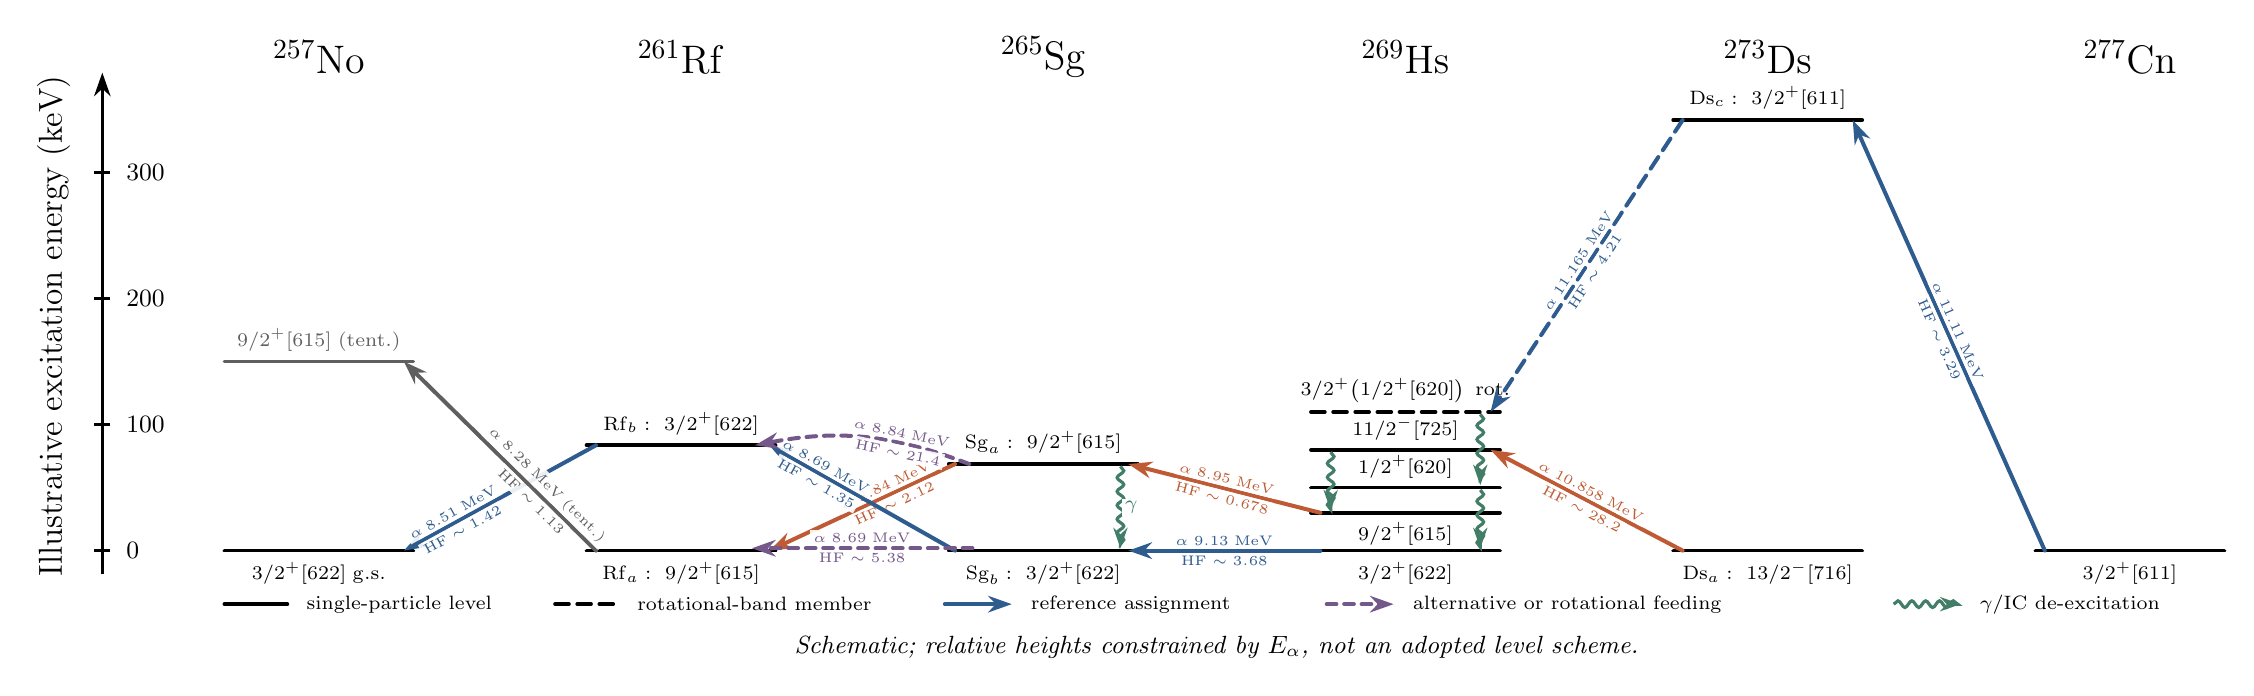
\begin{tikzpicture}[
    x=1cm,
    y=1cm,
    level/.style={
        line width=1.35pt,
        line cap=round
    },
    rotational level/.style={
        level,
        dash pattern=on 5pt off 3pt
    },
    transition/.style={
        -{Stealth[length=3.0mm,width=2.1mm]},
        line width=1.45pt,
        line cap=round
    },
    rotational transition/.style={
        transition,
        dash pattern=on 5pt off 3pt
    },
    alternative transition/.style={
        transition,
        dash pattern=on 3.5pt off 2.8pt
    },
    gamma/.style={
        decorate,
        decoration={
            snake,
            amplitude=1.20pt,
            segment length=5.0pt
        },
        -{Stealth[length=2.6mm,width=1.8mm]},
        line width=1.15pt
    },
    state/.style={
        font=\scriptsize,
        inner sep=1pt
    },
    nucleus/.style={
        font=\Large\bfseries
    },
    ticklabel/.style={
        font=\small
    },
    alphalabel/.style={
        font=\tiny,
        align=center,
        fill=white,
        fill opacity=0.90,
        text opacity=1,
        inner sep=1.2pt
    },
    hflabel/.style={
        alphalabel
    },
    note/.style={
        font=\scriptsize,
        align=center
    }
]

% ============================================================
% Muted scientific colors
% ============================================================

\definecolor{branchblue}{RGB}{47,92,143}
\definecolor{branchorange}{RGB}{190,91,52}
\definecolor{alternativepurple}{RGB}{117,88,138}
\definecolor{gammagreen}{RGB}{66,125,103}
\definecolor{tentativegray}{RGB}{95,95,95}

% ============================================================
% Illustrative excitation-energy coordinates
% ============================================================
%
% A common linear vertical scale is used.  The numerical choices are only
% one energy-consistent realization of the constraints in the accompanying
% Markdown document; they are not adopted excitation energies.

\def\yZero{1.45}
\def\eScale{0.016}

\pgfmathsetmacro{\yNoTent}{\yZero + 150.0*\eScale}

\pgfmathsetmacro{\yRfB}{\yZero + 83.6*\eScale}

\pgfmathsetmacro{\ySgA}{\yZero + 68.7*\eScale}

\pgfmathsetmacro{\yHsNine}{\yZero + 30.0*\eScale}
\pgfmathsetmacro{\yHsBandHead}{\yZero + 50.0*\eScale}
\pgfmathsetmacro{\yHsLong}{\yZero + 80.0*\eScale}
\pgfmathsetmacro{\yHsBandThree}{\yZero + 110.0*\eScale}

% Delta_E(Ds) = 311.6 + (110 - 80) = 341.6 keV.
\pgfmathsetmacro{\yDsExcited}{\yZero + 341.6*\eScale}

% Axis ticks
\pgfmathsetmacro{\yOneHundred}{\yZero + 100*\eScale}
\pgfmathsetmacro{\yTwoHundred}{\yZero + 200*\eScale}
\pgfmathsetmacro{\yThreeHundred}{\yZero + 300*\eScale}

% ============================================================
% Horizontal coordinates: decay direction is from right to left
% ============================================================

\def\xAxis{0.00}

\def\xNoL{1.55}
\def\xNoR{3.95}

\def\xRfL{6.15}
\def\xRfR{8.55}

\def\xSgL{10.75}
\def\xSgR{13.15}

\def\xHsL{15.35}
\def\xHsR{17.75}

\def\xDsL{19.95}
\def\xDsR{22.35}

\def\xCnL{24.55}
\def\xCnR{26.95}

% ============================================================
% Illustrative excitation-energy axis
% ============================================================

\draw[line width=1.05pt]
    (\xAxis,1.15)
    --
    (\xAxis,7.15);

\draw[
    -{Stealth[length=3.0mm,width=2.1mm]},
    line width=1.05pt
]
    (\xAxis,7.15)
    --
    (\xAxis,7.52);

\foreach \yy/\lab in {
    \yZero/0,
    \yOneHundred/100,
    \yTwoHundred/200,
    \yThreeHundred/300
}{
    \draw[line width=1.0pt]
        (\xAxis-0.10,\yy)
        --
        (\xAxis+0.10,\yy);
    \node[ticklabel,anchor=west]
        at (\xAxis+0.18,\yy)
        {\lab};
}

\node[font=\large,rotate=90]
    at (\xAxis-0.62,4.30)
    {Illustrative excitation energy (keV)};

% ============================================================
% Nucleus labels
% ============================================================

\node[nucleus] at ({(\xNoL+\xNoR)/2},7.72)
    {$^{257}\mathrm{No}$};
\node[nucleus] at ({(\xRfL+\xRfR)/2},7.72)
    {$^{261}\mathrm{Rf}$};
\node[nucleus] at ({(\xSgL+\xSgR)/2},7.72)
    {$^{265}\mathrm{Sg}$};
\node[nucleus] at ({(\xHsL+\xHsR)/2},7.72)
    {$^{269}\mathrm{Hs}$};
\node[nucleus] at ({(\xDsL+\xDsR)/2},7.72)
    {$^{273}\mathrm{Ds}$};
\node[nucleus] at ({(\xCnL+\xCnR)/2},7.72)
    {$^{277}\mathrm{Cn}$};

% ============================================================
% 257No levels
% ============================================================

\draw[level]
    (\xNoL,\yZero)
    --
    (\xNoR,\yZero);
\node[state,anchor=north]
    at ({(\xNoL+\xNoR)/2},\yZero-0.10)
    {$3/2^{+}[622]\;\mathrm{g.s.}$};

\draw[level,tentativegray]
    (\xNoL,\yNoTent)
    --
    (\xNoR,\yNoTent);
\node[state,anchor=south,tentativegray]
    at ({(\xNoL+\xNoR)/2},\yNoTent+0.09)
    {$9/2^{+}[615]\;\mathrm{(tent.)}$};

% ============================================================
% 261Rf levels
% ============================================================

\draw[level]
    (\xRfL,\yZero)
    --
    (\xRfR,\yZero);
\node[state,anchor=north]
    at ({(\xRfL+\xRfR)/2},\yZero-0.10)
    {$\mathrm{Rf}_{a}:\ 9/2^{+}[615]$};

\draw[level]
    (\xRfL,\yRfB)
    --
    (\xRfR,\yRfB);
\node[state,anchor=south]
    at ({(\xRfL+\xRfR)/2},\yRfB+0.09)
    {$\mathrm{Rf}_{b}:\ 3/2^{+}[622]$};

% ============================================================
% 265Sg levels
% ============================================================

\draw[level]
    (\xSgL,\yZero)
    --
    (\xSgR,\yZero);
\node[state,anchor=north]
    at ({(\xSgL+\xSgR)/2},\yZero-0.10)
    {$\mathrm{Sg}_{b}:\ 3/2^{+}[622]$};

\draw[level]
    (\xSgL,\ySgA)
    --
    (\xSgR,\ySgA);
\node[state,anchor=south]
    at ({(\xSgL+\xSgR)/2},\ySgA+0.09)
    {$\mathrm{Sg}_{a}:\ 9/2^{+}[615]$};

% ============================================================
% 269Hs levels
% ============================================================

\draw[level]
    (\xHsL,\yZero)
    --
    (\xHsR,\yZero);
\node[state,anchor=north]
    at ({(\xHsL+\xHsR)/2},\yZero-0.10)
    {$3/2^{+}[622]$};

\draw[level]
    (\xHsL,\yHsNine)
    --
    (\xHsR,\yHsNine);
\node[state,anchor=north]
    at ({(\xHsL+\xHsR)/2},\yHsNine-0.08)
    {$9/2^{+}[615]$};

\draw[level]
    (\xHsL,\yHsBandHead)
    --
    (\xHsR,\yHsBandHead);
\node[state,anchor=south]
    at ({(\xHsL+\xHsR)/2},\yHsBandHead+0.08)
    {$1/2^{+}[620]$};

\draw[level]
    (\xHsL,\yHsLong)
    --
    (\xHsR,\yHsLong);
\node[state,anchor=south]
    at ({(\xHsL+\xHsR)/2},\yHsLong+0.08)
    {$11/2^{-}[725]$};

\draw[rotational level]
    (\xHsL,\yHsBandThree)
    --
    (\xHsR,\yHsBandThree);
\node[state,anchor=south]
    at ({(\xHsL+\xHsR)/2},\yHsBandThree+0.08)
    {$3/2^{+}\!\left(1/2^{+}[620]\right)\;\mathrm{rot.}$};

% ============================================================
% 273Ds levels
% ============================================================

\draw[level]
    (\xDsL,\yZero)
    --
    (\xDsR,\yZero);
\node[state,anchor=north]
    at ({(\xDsL+\xDsR)/2},\yZero-0.10)
    {$\mathrm{Ds}_{a}:\ 13/2^{-}[716]$};

\draw[level]
    (\xDsL,\yDsExcited)
    --
    (\xDsR,\yDsExcited);
\node[state,anchor=south]
    at ({(\xDsL+\xDsR)/2},\yDsExcited+0.10)
    {$\mathrm{Ds}_{c}:\ 3/2^{+}[611]$};

% ============================================================
% 277Cn working level
% ============================================================

\draw[level]
    (\xCnL,\yZero)
    --
    (\xCnR,\yZero);
\node[state,anchor=north]
    at ({(\xCnL+\xCnR)/2},\yZero-0.10)
    {$3/2^{+}[611]$};

% ============================================================
% Alpha-decay branches, directed from right to left
% ============================================================

% 277Cn -> 273Ds_c.  The rejected l_alpha=5 branch is omitted.
\draw[transition,branchblue]
    (\xCnL+0.12,\yZero)
    --
    node[alphalabel,sloped,above] {\alphaval{11.11}}
    node[hflabel,sloped,below] {\hfval{3.29}}
    (\xDsR-0.12,\yDsExcited);

% 273Ds_c -> rotational member of the 1/2+[620] band: dashed.
\draw[rotational transition,branchblue]
    (\xDsL+0.12,\yDsExcited)
    --
    node[alphalabel,sloped,above] {\alphaval{11.165}}
    node[hflabel,sloped,below] {\hfval{4.21}}
    (\xHsR-0.12,\yHsBandThree);

% 273Ds_a -> 269Hs 11/2-[725].
\draw[transition,branchorange]
    (\xDsL+0.12,\yZero)
    --
    node[alphalabel,sloped,above] {\alphaval{10.858}}
    node[hflabel,sloped,below] {\hfval{28.2}}
    (\xHsR-0.12,\yHsLong);

% 269Hs -> 265Sg.
\draw[transition,branchblue]
    (\xHsL+0.12,\yZero)
    --
    node[alphalabel,above] {\alphaval{9.13}}
    node[hflabel,below] {\hfval{3.68}}
    (\xSgR-0.12,\yZero);

\draw[transition,branchorange]
    (\xHsL+0.12,\yHsNine)
    --
    node[alphalabel,sloped,above] {\alphaval{8.95}}
    node[hflabel,sloped,below] {\hfval{0.678}}
    (\xSgR-0.12,\ySgA);

% Preferred diagonal Sg -> Rf reference assignments.
\draw[transition,branchorange]
    (\xSgL+0.08,\ySgA)
    --
    node[alphalabel,sloped,above,pos=0.35] {\alphaval{8.84}}
    node[hflabel,sloped,below,pos=0.35] {\hfval{2.12}}
    (\xRfR-0.08,\yZero);

\draw[transition,branchblue]
    (\xSgL+0.08,\yZero)
    --
    node[alphalabel,sloped,above,pos=0.72] {\alphaval{8.69}}
    node[hflabel,sloped,below,pos=0.72] {\hfval{1.35}}
    (\xRfR-0.08,\yRfB);

% Alternative Sg_a -> Rf_b assignment.
\draw[alternative transition,alternativepurple]
    (\xSgL+0.26,\ySgA)
    to[bend right=16]
    node[alphalabel,sloped,above,pos=0.32] {\alphaval{8.84}}
    node[hflabel,sloped,below,pos=0.32] {\hfval{21.4}}
    (\xRfR-0.26,\yRfB);

% Alternative Sg_b -> Rf_a assignment.
\draw[alternative transition,alternativepurple]
    (\xSgL+0.30,\yZero+0.03)
    --
    node[alphalabel,above] {\alphaval{8.69}}
    node[hflabel,below] {\hfval{5.38}}
    (\xRfR-0.30,\yZero+0.03);

% 261Rf -> 257No.
\draw[transition,branchblue]
    (\xRfL+0.12,\yRfB)
    --
    node[alphalabel,sloped,above,pos=0.72] {\alphaval{8.51}}
    node[hflabel,sloped,below,pos=0.72] {\hfval{1.42}}
    (\xNoR-0.12,\yZero);

\draw[transition,tentativegray]
    (\xRfL+0.12,\yZero)
    --
    node[alphalabel,sloped,above,pos=0.30]
        {\alphaval{8.28}\;\ensuremath{(\mathrm{tent.})}}
    node[hflabel,sloped,below,pos=0.30] {\hfval{1.13}}
    (\xNoR-0.12,\yNoTent);

% ============================================================
% Gamma / internal-conversion de-excitation
% ============================================================

% 269Hs high-spin and low-spin cascades.
\draw[gamma,gammagreen]
    (\xHsL+0.25,\yHsLong-0.03)
    --
    (\xHsL+0.25,\yHsNine+0.03);

\draw[gamma,gammagreen]
    (\xHsR-0.25,\yHsBandThree-0.03)
    --
    (\xHsR-0.25,\yHsBandHead+0.03);

\draw[gamma,gammagreen]
    (\xHsR-0.25,\yHsBandHead-0.03)
    --
    (\xHsR-0.25,\yZero+0.03);

% Sg_a -> Sg_b de-excitation.
\draw[gamma,gammagreen]
    (\xSgR-0.22,\ySgA-0.03)
    --
    node[state,fill=white,inner sep=1pt,right] {$\gamma$}
    (\xSgR-0.22,\yZero+0.03);

% ============================================================
% Legend and required schematic qualification
% ============================================================

\draw[level] (1.55,0.77) -- (2.35,0.77);
\node[note,anchor=west] at (2.47,0.77) {single-particle level};

\draw[rotational level] (5.75,0.77) -- (6.55,0.77);
\node[note,anchor=west] at (6.67,0.77) {rotational-band member};

\draw[transition,branchblue] (10.70,0.77) -- (11.55,0.77);
\node[note,anchor=west] at (11.67,0.77) {reference assignment};

\draw[alternative transition,alternativepurple]
    (15.55,0.77) -- (16.40,0.77);
\node[note,anchor=west] at (16.52,0.77)
    {alternative or rotational feeding};

\draw[gamma,gammagreen] (22.75,0.77) -- (23.60,0.77);
\node[note,anchor=west] at (23.72,0.77) {$\gamma$/IC de-excitation};

\node[note,font=\small\itshape]
    at (14.15,0.22)
    {Schematic; relative heights constrained by $E_{\alpha}$, not an adopted level scheme.};

\end{tikzpicture}

\end{document}
